\sectionmark{Wachstum der Bakterien I}

\section{Wachstum der Bakterien I}
\begin{enumerate}
	\item Nennen Sie fünf Makroelemente, die alle Organismen zum Leben brauchen und deren Quellen für Bakterien (dabei sollte mindestens 1 Metall sein)!

		Einige, für Mikroorganismen wichtige Markoelemente und ihre Quellen sind in Tabelle \ref{tab:makroelemente}
		beschrieben.
		\begin{table}[h!]
		\begin{center}
		\begin{tabular}{l l} 
		\toprule
		Element	&	Bereitstellung	in der Natur \\
		\midrule
		C			&	\ce{CO2}, organische Stoffe \\
		H			&	\ce{H2O}, organische Stoffe \\
		O			&	\ce{H2O}, \ce{O2}, organische Stoffe \\
		N			&	\ce{NH3}, \ce{NO3-}, \ce{N2}, organische Stoffe \\
		P			&	Phosphat \\
		S			&	\ce{H2S}, organische Stoffe, Sulfide \\
		\midrule
		K			&	Kaliumsalze \\
		Mg			&	Magnesiumsalze \\
		Na			&	\ce{NaCl}, Natriumsalze \\
		Ca			&	Salze \\
		\midrule
		Fe			&	\ce{FeS}, Eisensalze \\
		\bottomrule
		\end{tabular}
		\caption{Mikroelementen und ihre Quellen für Mikroorganismen}
		\label{tab:makroelemente}
		\end{center}
		\end{table}

	\item Nennen Sie einige Mikroelemente und erklären Sie, wofür diese Elemente benötigt werden!
	
		Einige, für Mikroorganismen wichtige Mirkoelemente und ihre Funktionsort sind in Tabelle \ref{tab:mikroelemente}
		beschrieben.
		\begin{table}[h!]
		\begin{center}
		\begin{tabular}{l l} 
		\toprule
			Element	&	Funktion in der Zelle \\
			\midrule
			Co			&	\ce{B12}, Transcaboxylase \\
			Cu			&	Atmung, CytC-Oxidase, Photosynthese\\
			Mn			&	Photosystem II, Superoxiddismutase \\
			Mo			&	Nitrogenase, Nitratreduktase, Formiat-DHG \\
			Ni			&	Hydorgenase, Co-F430 (Methanogene), \ce{CO}-Dehydrogenase \\
			Se			&	Formiat-DHG, Hydrogenase\\
			W			&	Formiat-DHG \\
			V			&	Vanadium-Nitrogenase \\
			Zn			&	Alkohol-DHG, RNA-/DNA-Polymerase \\
			Fe			&	Cytochrome, Katalasen, FeS-Proteine, alle Nitrogenasen \\
		\bottomrule
		\end{tabular}
		\label{tab:mikroelemente}
		\caption{Mikroelementen und ihre Quellen für Mikroorganismen}
		\end{center}
		\end{table}

	\item Stellen Sie sich vor, sie kultivieren \emph{E. coli}! Sie starten eine Kultur mit 3000 Zellen und kultivieren sie dann unter optimalen Bedingungen für 12 Stunden. Zeichnen Sie schematisch die Wachstumskurve dieser Kultur (bitte denken Sie an die Achsenbeschriftung und die Skalierung)!

		In Abbildung \ref{fig:ecoliplot} ist die Anzahl der Zellen von \emph{E. coli} innerhalb der ersten 12 Stunden aufgetragen.	
		\begin{figure}[ht!]
		\leavevmode
		\begin{center}
		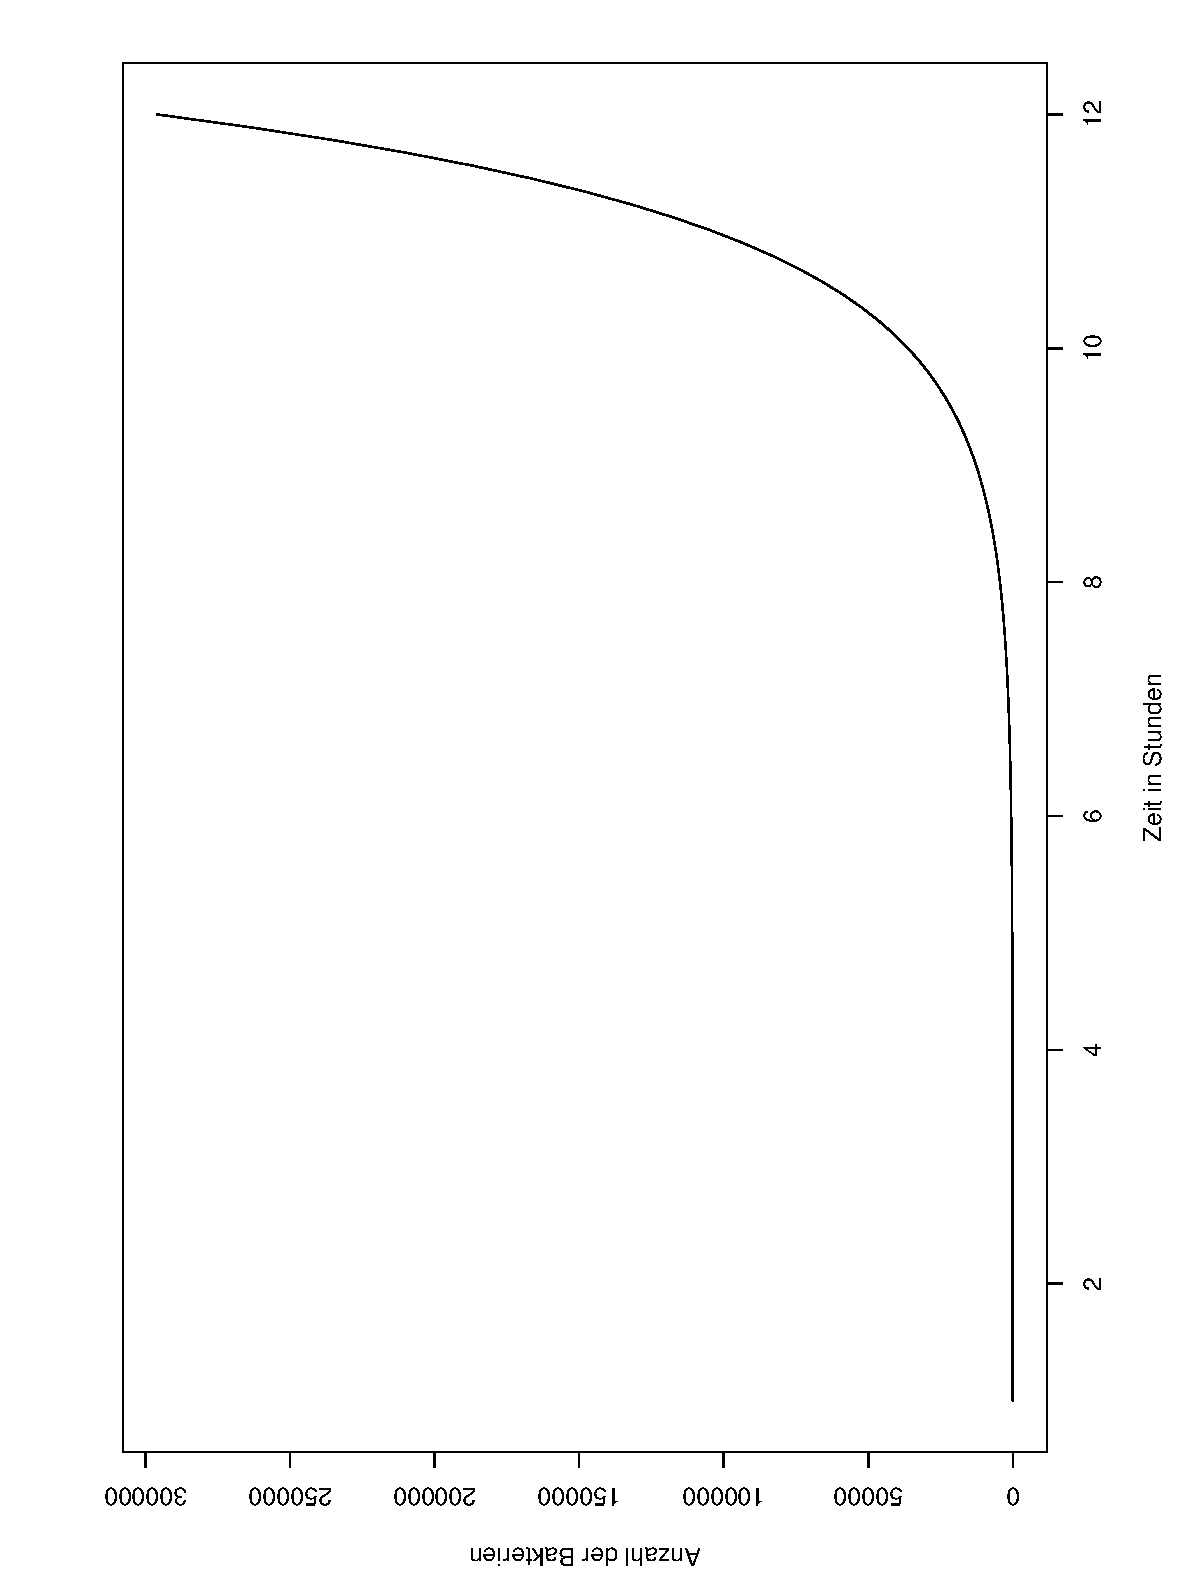
\includegraphics[scale=0.5]{./pictures/ecoli_plot.pdf}		% TODO:schoener machen :\
		\end{center}
		\caption{\slshape{Wachstum von E. coli}}
		\label{fig:ecoliplot}
		\end{figure}

	\item Die einfachste Methode zur Messung des Wachstums ist die Trübungsmessung. Würden Sie diese Methode anwenden, wenn Sie mit \emph{Streptomyceten} arbeiten? Begründen Sie Ihre Antwort!
		Da \emph{Streptomyceten} nicht dispers wachsen,
		ist die Messung des Wachstums mit Trübung	nicht möglich.

		Bei der Trübmessung wird gemessen wieviel des auf die Kultur eingestrahlten Lichtes diese durchdringt.
		Durch zunehmmende Zellzahlen nimmt der Anteil des durch die Kultur Absorbierten Lichtes ab.
		Um diese Methode anwenden zukönnen,
		müssen die Mikroorganismen jedoch dispers wachsen.
		Das heisst keine Zusammenhängenden Strukturen ausbilden. % Todo - Brock überprüfen

	\item Die Proteine FtsZ und MreB sind für die Zellteilung sehr wichtig. Wozu würde die Zerstörung dieser beiden Gene in \emph{E. coli} führen?
		Das Protein \emph{FtsZ}, ``Filamentus temperatur sensitive mutant Z'',
		ist entscheidenen am Prozess der Zellteilung beteiligt.
		Nach der Elongation der Zelle,
		bilden \emph{FtsZ}-Proteine das sogenannte Divisom und,
		trennen die Zelle in zwei Hälften.
		Dabei interagiert der \emph{FtsZ}-Ring mit den bereits duplizierten Nukleoid.
		Entlang des Ringes wird schließlich die neue Zellwand gebildet.
		Diese ist beim Abschnüren der entstehenden Tochterzellen bereits gebilder,
		um die strukturelle Integrität der Zellen zu erhalten.	% todo -pics

		\begin{figure}
		\centering
		\subfloat[FstZ]{\label{fig:fstz}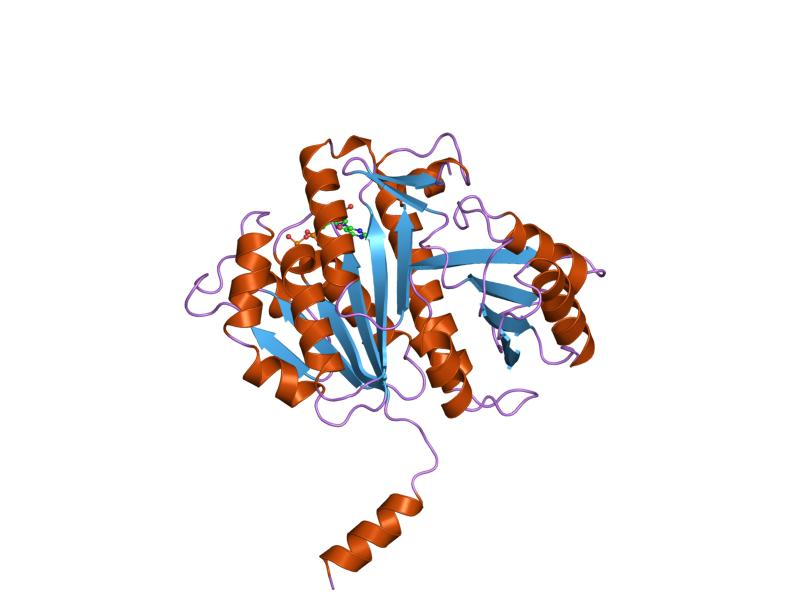
\includegraphics[width=0.44\textwidth]{./pictures/ftsz_800}}
		\subfloat[MreB]{\label{fig:mreb}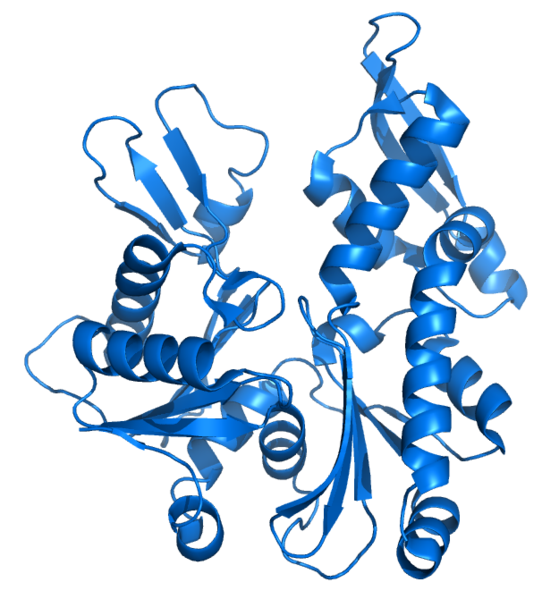
\includegraphics[width=0.25\textwidth]{./pictures/MreB_500}}
		\subfloat[Actin]{\label{fig:fstz}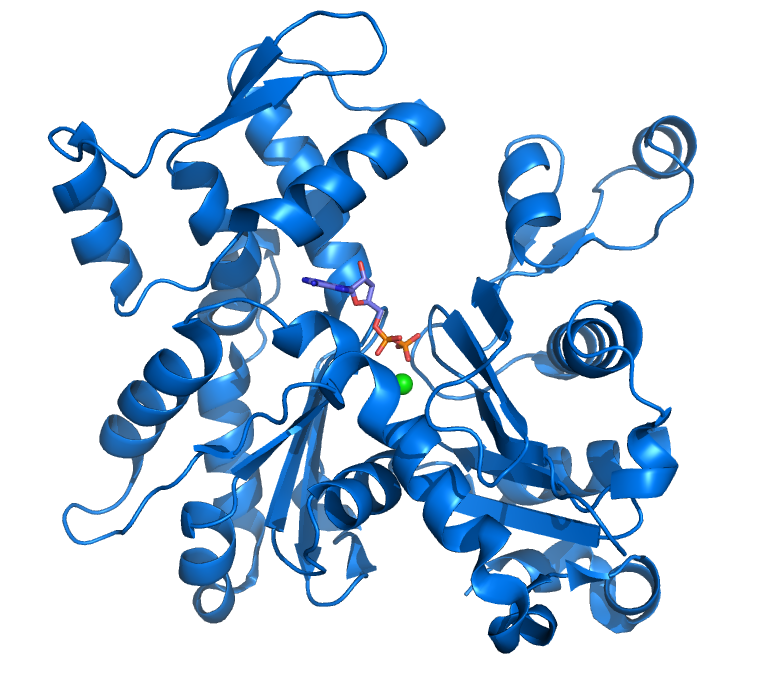
\includegraphics[width=0.3\textwidth]{./pictures/actin_762}}
		\caption{\slshape{Tertiärstruktur von Proteinen mit hoher Beduetung für die Zellteilung und Cytoskelett in \emph{E. coli}}}
		\label{fig:ecoli_proteins}
		\end{figure}

		Bei \emph{MreB} handelt es sich um ein dem \emph{Actin} homolgen Protein.
		Diese Proteine sind mit dem Cytoskellete der Zellen assoziert.
		\emph{MreB} bilder spiralige Bänder innerhalb der cytoplasmatischen Membran.
		In kokkenförmigen Bakterien ist \emph{MreB} nicht gefunden worden.
		Erst durch dieses Protein können Vibrionen, Stäbchen und Spirillen endstehen.
		Bakterien mit einem Mutanten sind jedoch kokkoid.

		Die Tertiärstrukturen der der Proteine sind in Abbildung \ref{fig:ecoli_proteins} dargestellt.
		
	\item Bei steigender Temperatur steigt die Wachstumsrate von Bakterien bis zum Optimum langsam an, dann fällt Sie schnell ab. Begründen Sie diesen Kurvenverlauf!

		Die Enzymatische Aktivität steigt stetig bedingt durch RGT-Regel.
		Übersteigt die Temperatur jedoch eine bestimmte,
		für jeden Mikroorganismus spezifische,
		Schwelle, denaturieren wichtige Proteine.
		Da diese nun nichtmehr ihrer Funktion erfüllen,
		können sich die Mikroorganismen nicht weiter vermehren.
		Zusätzlich wird ab einer spezifischen Temperatur die Membran instabil.

		Die Temperatur darf aber auch eine spezifische Temperatur nicht unterschreiten.
		Bei niedrigen Temperaturen verliert die Membran ihre Fluidität und
		Transportprozesse laufen zu langsam ab so das die Zellen nicht wachsen können.
		Die Minimal-, Optimal- und Maximal-Temperatur werden auch als Kardinaltemperaturen
		bezeichnet und sind in Tabelle \ref{tab:ecolikardinal} für \emph{E. coli} aufgeführt.

		\begin{table}[h!]
		\begin{center}
		\begin{tabular}{l l l} 
		\toprule
		Kardinaltemperatur	&	Wert	&	Begrenzender Faktor\\
		\midrule
		Minimaltemperatur		&	8\textdegree C	&	Membranzustand, RNA \\
		Optimaltemperatur		&	39\textdegree C	&	Optimale Bedingungnen	\\
		Maximaltemperatur		&	48\textdegree C	&	Inaktivierung wichtiger Proteine \\
		\bottomrule
		\end{tabular}
		\caption{Kardinaltemperaturen von \emph{E. coli}}
		\label{tab:ecolikardinal}
		\end{center}
		\end{table}

	\item Warum die Anpassung an niedrige Temperaturen bei Lipiden besonders wichtig? Nennen Sie einige Möglichkeiten dafür!

		Lipide befinden sich in Zellen hauptsächlich in der Membran.
		Durch Kälte sinkt die Fluidität der Membran und sie wird gelartig,
		was die Lebensvorgänge der Mikrooorganismen stark beeinträchtigt.
		Durch eingelagerte Stoffe wie Cholesterin bliebt die Membran fluide.
		Zusäzlich haben an Kälte angepasst Mikroorganismen einen höheren Anteil an ungesättigten Fettsäuren
		in der Membran.
\end{enumerate}
